\section{Project Management}\label{section:project_management}

\subsection{Version Control}\label{subsection:version_control}

\lettrine{P}{acket} Courier was developed using Git\cite{git} as a version control system and the code repository is
hosted on GitHub\cite{github, packet_courier} at \url{https://github.com/thelukethorpe/packet_courier}. There is no
special reason for either of these choices; they are simply industry standards being used for a project that doesn't
innately demand bespoke tooling (unlike data-heavy ventures such as game development, which might benefit from a tool
like Perforce\cite{perforce, perforce_vs_git}).

\subsection{Ticket Tracking}\label{subsection:ticket_tracking}

\lettrine{G}{itHub} Issues\cite{github_issues} powers Packet Courier's ticket tracking. Tickets, or \emph{issues}, as
per the GitHub nomenclature, are categorised based on one or more of the following custom tags:
\begin{itemize}
    \item \textbf{Bug:} \emph{Something isn't working.}
    \item \textbf{CI:} \emph{Change to pipeline.}
    \item \textbf{Documentation:} \emph{Improvements or additions to documentation.}
    \item \textbf{Feature:} \emph{New feature or request.}
    \item \textbf{Optimization:} \emph{Improvements in performance.}
    \item \textbf{Refactor:} \emph{Tech-debt, structural change of quality-of-life improvement.}
    \item \textbf{Testing:} \emph{Improvements or additions to test suite.}
    \item \textbf{Won't Fix:} \emph{This will not be worked on.}
\end{itemize}

Issues are further organised using a Kanban board\cite{kanban_board}. As the \emph{documentation} tag suggests,
this board is not only used for development purposes, in fact, it has been used to help manage the project
holistically, including the writing of this very report, as shown in
Figure~\ref{fig:chapter_4_implementation-github_kanban_board}.

\begin{figure}[!h]
    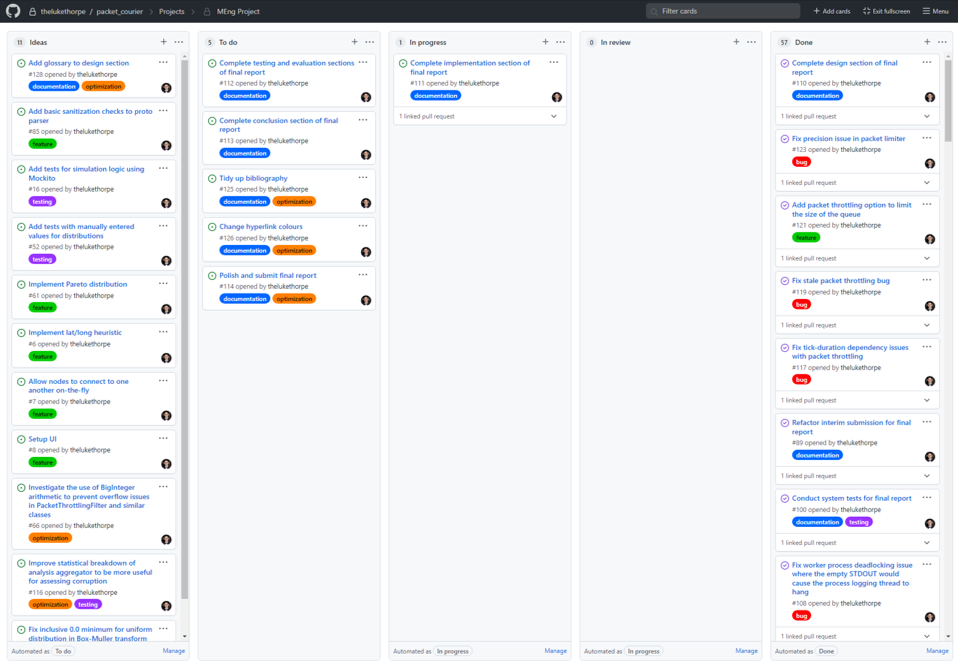
\includegraphics[width=\textwidth]{images/chapter_4_implementation/github_kanban_board}
    \centering~\caption{Packet Courier's Project Kanban Board\cite{packet_courier}.}
    \label{fig:chapter_4_implementation-github_kanban_board}
\end{figure}

Pull-requests are opened for every merge to the \texttt{main} branch and linked to the associated ticket number.
Branches are named with a uniform and consistent structure, prefixed by the issue number followed by a brief subtitle
of the ticket delimited by hyphens. Despite being an individual project, this repository has been maintained to
industry standards of software engineering practices for organisational reasons, and has in turn benefited massively
from it.

\begin{figure}[!h]
    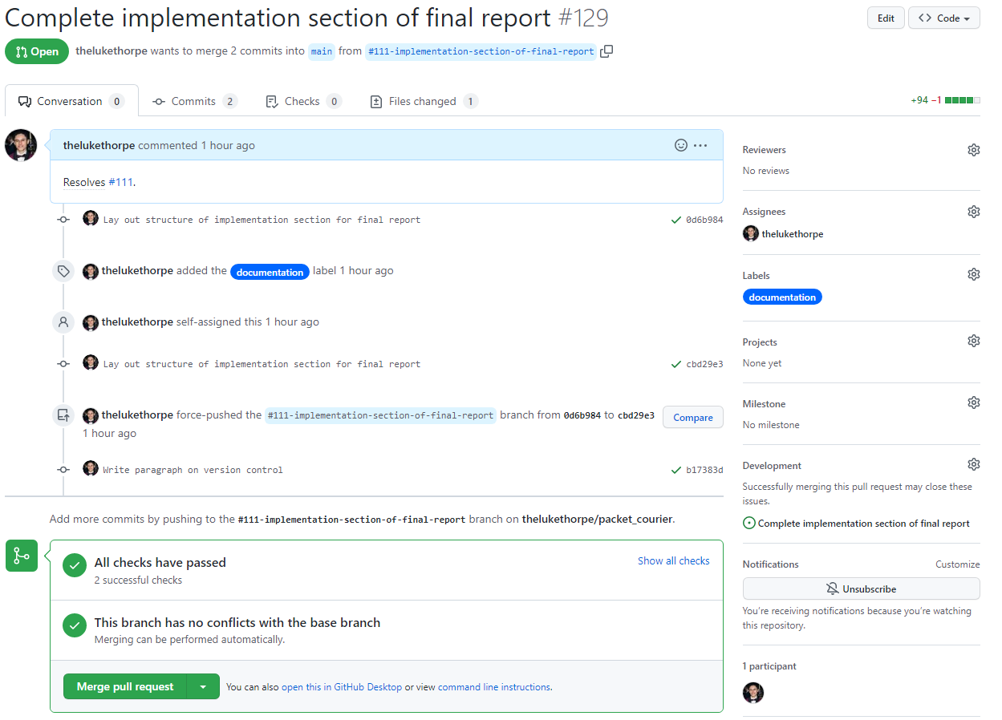
\includegraphics[width=\textwidth]{images/chapter_4_implementation/github_pull_request}
    \centering~\caption{An example of a pull-request in the Packet Courier repository\cite{packet_courier}.}
    \label{fig:chapter_4_implementation-github_pull_request}
\end{figure}

\newpage

\subsection{Programming Languages}\label{subsection:programming_languages}

\lettrine{J}{ava} 8\cite{java_8} was chosen as the foundational language for Packet Courier due to:
\begin{itemize}
    \item Its excellent breadth of supported platforms\cite{java_8_support}, which lends itself well to objective 4.a).
    \item The vast number of popular and easily importable libraries available to it\cite{java_relevance}.
    \item Its object-oriented nature, which maps nicely onto the abstract semantics laid out in
    Section~\ref{section:high_level_architecture}.
    \item Its relatively high levels of time-efficiency, as shown in
    Figure~\ref{fig:chapter_4_implementation-programming_language_comparison}.
    \item Its suite of concurrency abstractions\cite{java_util_concurrent}.
\end{itemize}

\begin{figure}[!h]
    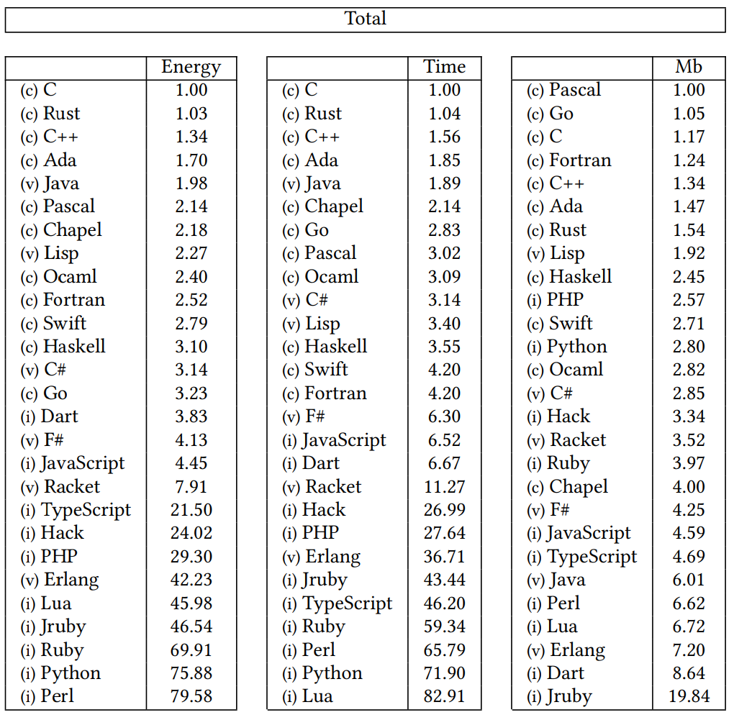
\includegraphics[width=\textwidth]{images/chapter_4_implementation/programming_language_comparison}
    \centering~\caption{A comparison of programming languages based on energy usage, time and memory
    efficiency\cite{programming_language_efficiency}.}
    \label{fig:chapter_4_implementation-programming_language_comparison}
\end{figure}

Although languages such as C and C++ outperform Java across all metrics displayed by
Figure~\ref{fig:chapter_4_implementation-programming_language_comparison}, they are needlessly low-level to the point
where it would likely become a hindrance. Even a cursory investigation into the nature of socket programming in C++
revealed a perfect case study as to the benefits of Java for a problem statement like Packet Courier's. It turns out
that Windows does not natively support the standard C++ socket specification, \texttt{sys/socket.h}, meaning that
\texttt{winsock2.h} must be used instead\cite{socket_vs_winsock}. This would then mean either going to the effort of
implementing two different platform-dependent solutions, or using a library that promises platform agnosticism. There
are many such libraries however\cite{c++_socket_libraries}, placing a substantial research burden on the development
of what should be a fairly simple component. C++ furthermore has been shown to have several non-trivial cross-platform
and cross-compiler discrepancies for even the most basic code\cite{c++_cross_compiler_differences,
    c++_statistical_differences, c++_random_differences, c++_filesystem_differences}.

A key benefit of Java is that it smooths out cross-platform issues, providing developers with a clean, uniform and
highly reliable set of semantics that transcend the nuances of the native operating system and hardware
micro-architecture. Indeed, Java handily has a \texttt{DatagramSocket} class\cite{java_DatagramSocket} which has
proven extremely useful in implementing Packet Courier's standalone emulator. In this way, external Java libraries
are only called-in for more heavyweight or highly specific work, as opposed to routine or menial implementations.

Java also strikes a Goldilocks-esque balance\cite{goldilocks_effect} between low-level languages like C++ and
languages that are arguably even more abstract than Java, such as Python. Whilst Packet Courier does leverage Python
3\cite{python_3} for basic client-server scripts to demonstrate the functionality of the emulator, production code
consists exclusively of Java. Python's dynamic typing\cite{python_typing}, poor
performance\cite{programming_language_efficiency} and inefficient multi-threading and synchronisation
primitives\cite{python_gil} are the main reasons why it wasn't used more prominently within Packet Courier.

\subsection{Build and Dependency Management}\label{subsection:build_and_dependency_management}

\lettrine{P}{acket} Courier uses Apache Maven 3.6.3\cite{maven} to manage its build phases and dependencies. Maven is
convenient, lightweight, widely supported, boasts a huge repository of libraries\cite{maven_repository} and with a
single command can compile the project into a portable \texttt{.jar} file that can be used as an executable binary or
a Java library.

\subsubsection{JUnit 4}\label{subsubsection:junit_4}

JUnit 4\cite{juint4} is an industry standard for conducting tests in Java, with an estimated 30.7\% of Java projects on
GitHub using JUnit (according to a study done in 2013)\cite{java_library_popularity}. Naturally, the Packet Courier
unit tests are implemented using JUint 4.13 and are run on each Maven build.

\subsubsection{AssertJ}\label{subsubsection:assert_j}

\begin{lstlisting}[language=Java,caption={An example of a Packet Courier unit test using JUnit and AssertJ.},
    label={code:packet_test},captionpos=b]
public class PacketTest {
  // JUnit 4 test.
  @Test
  public void testPacketStringConversion() {
    String message = "hello there!";
    Packet messageAsPacket = Packet.of(message);
    // AssertJ assertion reads like an English sentence.
    assertThat(messageAsPacket.tryParse()).hasValue(message);
  }

  // Some more tests...
}
\end{lstlisting}


AssertJ\cite{assert_j} is used in conjunction with JUnit to provide unit tests with expressive, human-readable checks
as shown in Code-Snippet~\ref{code:packet_test}. The following paragraph from a \emph{JavaZone} article summarises
why AssertJ was favoured over the JUnit default assertion framework known as Hamcrest\cite{assert_j_vs_hamcrest}:
\begin{quote}
    \emph{``AssertJ is not as well-known as Hamcrest, but at the same time, its popularity has been growing pretty
    fast over the last few years. As opposed to Hamcrest’s classic assertion syntax, which was inherited from the
    default Java testing framework JUnit, the main idea of AssertJ is that it provides fluent syntax. The main goal
    of that is to improve code readability. It’s worth mentioning that AssertJ is a fork of the FEST Assert project,
        which was the first step of AssertJ creation.''}
\end{quote}

\subsubsection{Google Protocol Buffer}\label{subsubsection:google_protocol_buffer}

Google Protocol Buffer\cite{google_protobuf} is a multi-faceted library that is supported across multiple languages,
but is used by Packet Courier to parse configuration files into Java objects. There are many file parsing libraries
for specific file formats, such as Google Gson, a Java JSON parsing library\cite{google_gson}. The unique selling
point of Google Protocol Buffer is its neatly compartmentalised workflow:
\begin{enumerate}
    \item Write a \texttt{.proto} file that defines the expected file structure. See
    Code-Snippet~\ref{code:google_protocol_buffer_example} for an example.
    \item Compile the \texttt{.proto} file using Maven to generate the corresponding parse-tree in Java.
    \item Choose a parser such as \texttt{JsonFormat} to generate a parse-tree from an input file.
    \item Perform a semantic pass over the parse-tree, i.e.: completing basic sanity checks whilst converting the
    raw syntactic form of the parse-tree into something more abstract that can be assimilated into the core APIs.
\end{enumerate}

\begin{lstlisting}[language=protobuf2,style=protobuf,caption={An example of a \texttt{.proto} file that encodes for
an \texttt{AddressBook}. A data file that followed this syntactic structure could then be read into memory as an
\texttt{AddressBookProtos} Java class, ready for further abstraction.},
    label={code:google_protocol_buffer_example},captionpos=b]
    syntax = "proto2";

    package tutorial;

    option java_multiple_files = true;
    option java_package = "com.example.tutorial.protos";
    option java_outer_classname = "AddressBookProtos";

    message Person {
        optional string name = 1;
        optional int32 id = 2;
        optional string email = 3;

        enum PhoneType {
            MOBILE = 0;
            HOME = 1;
            WORK = 2;
        }

        message PhoneNumber {
            optional string number = 1;
            optional PhoneType type = 2 [default = HOME];
        }

        repeated PhoneNumber phones = 4;
    }

    message AddressBook {
        repeated Person people = 1;
    }
\end{lstlisting}

\subsubsection{Protocol Buffers Protobuf Maven Plugin}\label{subsubsection:protocol_buffers_protobuf_maven_plugin}

An unusual quirk of the Google Protocol Buffer Java library is that it doesn't compile all the requisite Java
classes into the final \texttt{.jar}; instead it assumes that they will be loaded into the project as part of a
separate library. The \texttt{protoc-jar-maven-plugin}\cite{protoc_jar_maven_plugin} helps to work around this issue
by adding an extra compilation step at compile time to plug this gap.

\subsection{Continuous Integration}\label{subsection:continuous_integration}

\lettrine{T}{he} Packet Courier repository uses GitHub actions\cite{github_actions} to implement a continuous
integration pipeline\cite{aws_ci} where code is linted and tested, both of which are done using Maven. Linting is
enforced using \texttt{fmt-maven-plugin}\cite{fmt_maven_plugin}, which provides users with an automated way to check
for and fix Java code that does not adhere to the Google Java Style Guide\cite{google_java_format,
    google_java_style_guide}. Testing is simply done via the Maven command:
\begin{quote}
    \texttt{mvn '-Dtest=**.*Test' test --no-transfer-progress}.
\end{quote}


\newpage


\section{API Overview}\label{section:api_overview}

\subsection{Repository Structure}\label{subsection:repository_structure}

\begin{figure}[!h]
    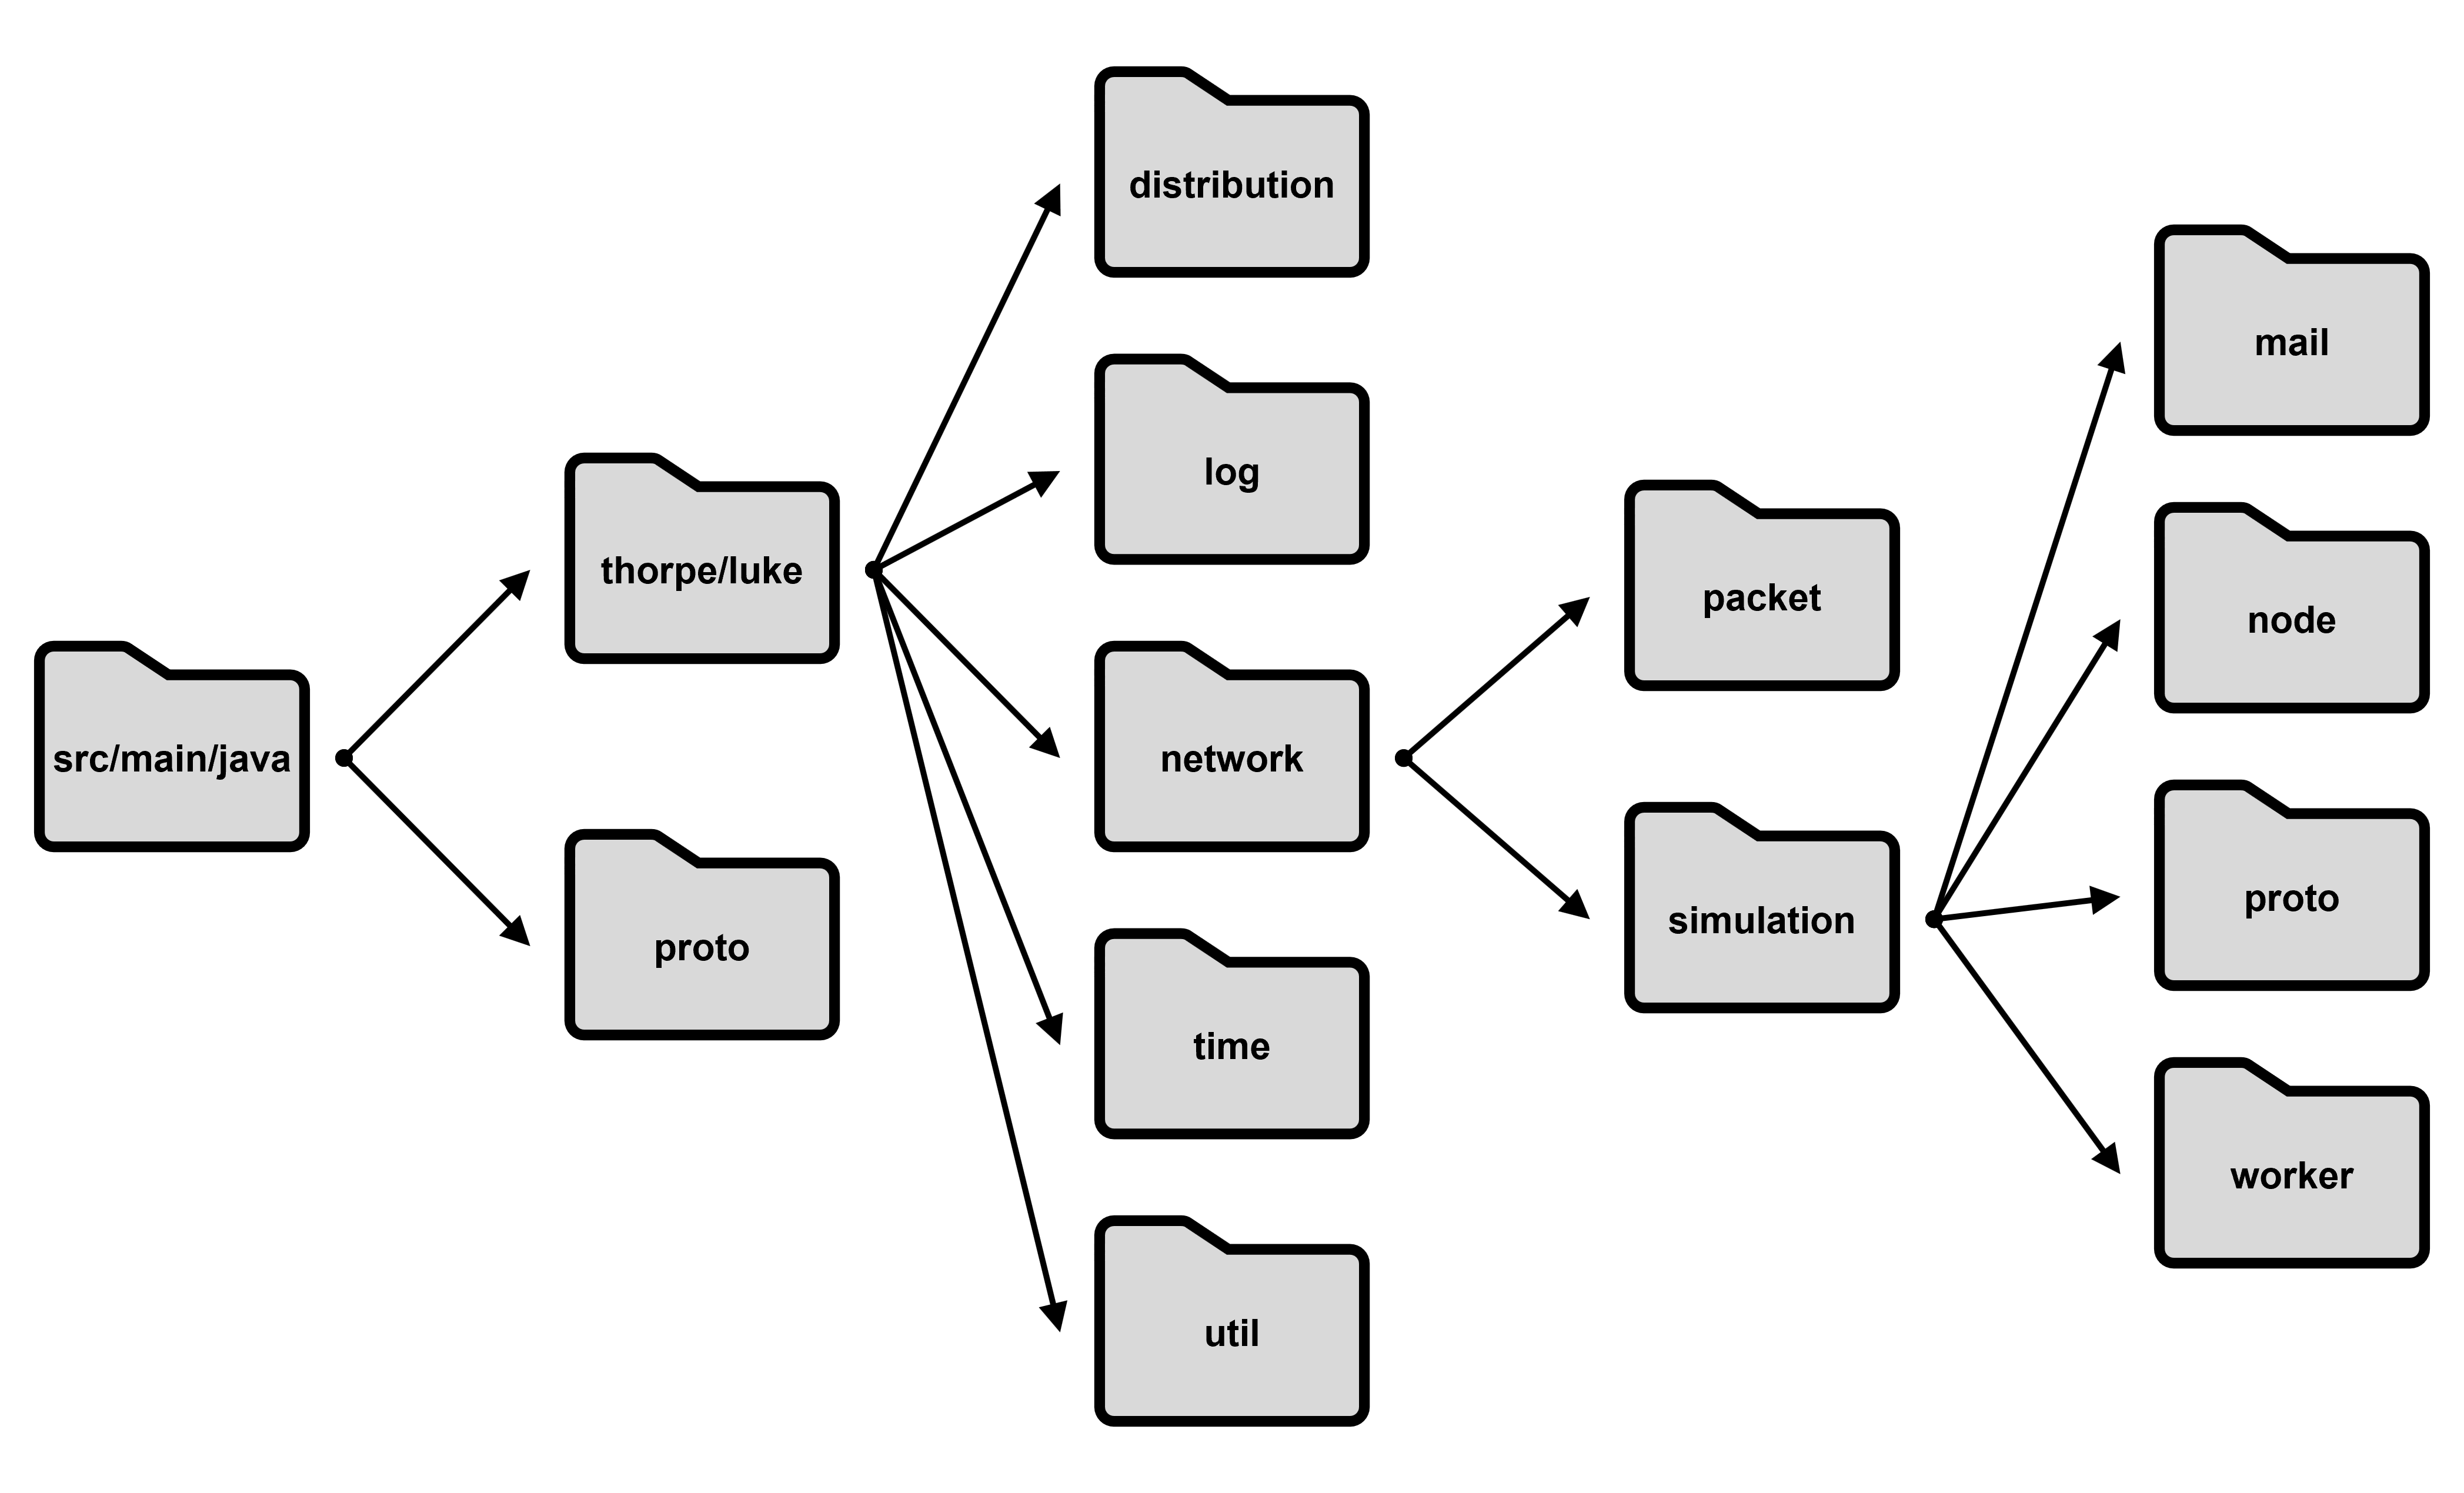
\includegraphics[width=\textwidth]{images/chapter_4_implementation/repository_structure}
    \centering~\caption{A diagram showing the directory tree of the repository's source code. The tests reside in
    \texttt{src/test} and are analogously structured.}
    \label{fig:chapter_4_implementation-repository_structure}
\end{figure}

\subsection{Statistical Distribution API}\label{subsection:statistical_distribution_api}

\lettrine{P}{acket} Courier supports the following statistical distributions:
\begin{itemize}
    \item Bernoulli
    \item Exponential
    \item Normal
    \item Poisson
    \item Continuous (Real) Uniform
    \item Discrete (Integer) Uniform
\end{itemize}

Each distribution implementation implements the \texttt{Distribution<T>} interface as shown in
Figure~\ref{fig:chapter_4_implementation-distribution_api_tree}, whereby type parameter \texttt{T} corresponds to the
type of value returned by the sampling function.

\begin{figure}[!h]
    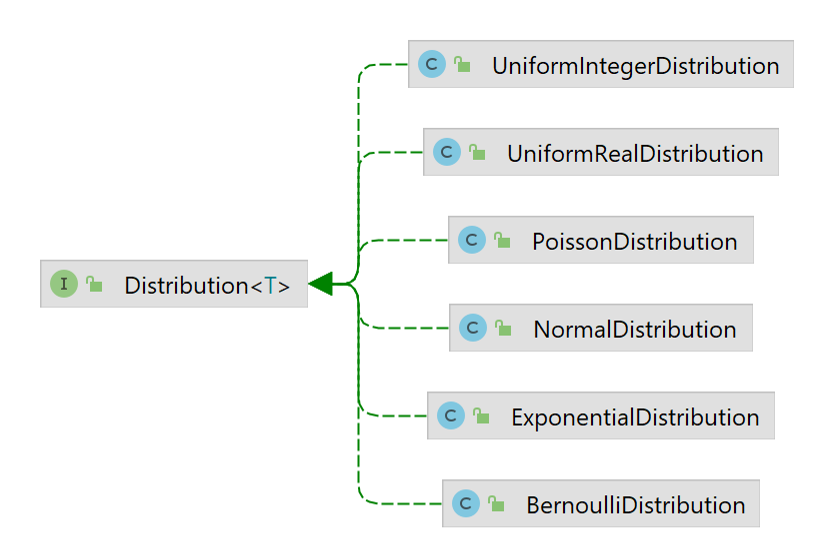
\includegraphics[width=0.65\textwidth]{images/chapter_4_implementation/distribution_api_tree}
    \centering~\caption{A diagram showing the class inheritance tree of the distribution API.}
    \label{fig:chapter_4_implementation-distribution_api_tree}
\end{figure}

As per Code-Snippet~\ref{code:distribution_inferface}, Packet Courier distributions adhere to the C++
distribution-generator pattern where the source of randomness, or \emph{generator}, is decoupled from the
parameterised statistical distribution that is being sampled from\cite{c++_random, c++_random_number_generation}. In
addition to the fact that decoupling is generally a good programming practice\cite{decoupling}, there are several
application-specific benefits to separating a distribution from its sampling
engine\cite{c++_random_number_generation_philosophy}:
\begin{itemize}
    \item Distributions are far more lightweight when they don't need to carry around a source of randomness. Indeed,
    there are a number of places within the Packet Courier codebase that create a temporary distribution to be
    sampled on-the-fly, as demonstrated in Code-Snippet~\ref{code:sample_from_event_duration_distribution}. If the
    distribution needed to be created with a source of randomness ahead of time, then this would likely result in
    much clumsier code. Of course, \texttt{Random} could be passed in as a constructor parameter, which wouldn't
    affect Code-Snippet~\ref{code:sample_from_event_duration_distribution} in any way, but it would make the
    distribution stateful.
    \item Stateful distributions are less useful and needlessly more prone to error. Indeed, a stateless distribution
    with no embedded source of randomness can be used in multiple different contexts or even across different
    threads. Consider a scenario where a Poisson distribution is being used to model the number of sheep in a field.
    Suppose a developer wanted to conduct two simulations for the same value of $\lambda$: one with pure randomness
    and the other with a correlation bias. Decoupling means that the same distribution can be used to conduct both
    experiments in parallel, whereas two of the same distribution would need to be created if the generator were
    embedded in the distribution. This is especially suboptimal in the case of a Poisson distribution,
    since the Packet Courier implementation generates a table for each distribution.
    \item Depending on how deeply embedded the random number generation engine is in the distribution, it could
    result in correlated results. For example, if two different normal distributions used a common seed for two
    different instances of \texttt{Random}, then the same sequence would be generated. As a consequence, the
    Box-Muller transform would generate the same values of $Z \sim \mathcal{N}(0,1)$\cite{box_muller_transform}. Even
    if the two distributions were parameterised differently, the two output sequences would still be linear functions
    of one another since $Z \sim \mathcal{N}(0,1) \implies \mu + \sigma Z \sim \mathcal{N}(\mu, \sigma^2)$. One might
    argue that this could be resolved by using different seeds for each distribution; notice that this becomes a
    nightmare very quickly, i.e.: coordinating the unique usage of seeds across all distributions, especially if
    seeds are user-parameterised. The much simpler solution is just to decouple random generation from
    stateless distributions.
\end{itemize}

\begin{lstlisting}[language=Java,caption={The \texttt{Distribution<T>} interface exactly as it appears in the
codebase.},label={code:distribution_inferface},captionpos=b]
public interface Distribution<T> {
  T sample(Random random);

  Double mean();

  Double variance();
}
\end{lstlisting}

\begin{lstlisting}[language=Java,caption={An example of a distribution being created and sampled on-the-fly with
arbitrary parameters.},label={code:sample_from_event_duration_distribution},captionpos=b]
public class SimulatedEventPipeline<Wrapper extends PacketWrapper<Wrapper>> implements PacketFilter<Wrapper> {
  // Random generator.
  private final Random random;

  // Method that generates the duration of a particular event,
  // as per the event-based semantics.
  private LocalDateTime sampleFromEventDurationDistribution(double meanDuration) {
    // Distribution is generated on-the-fly and used with
    // the class's in-house source of randomness.
    ExponentialDistribution eventDurationDistribution =
        new ExponentialDistribution(1.0 / meanDuration);
    long eventDuration = Math.round(eventDurationDistribution.sample(random));
    return now.plus(Duration.of(eventDuration, timeUnit));
  }

  // Rest of class...
}
\end{lstlisting}

Classes inheriting from \texttt{Distribution<T>} must also implement the \texttt{mean} and \texttt{variance} methods
for testing purposes. This will be discussed in more detail later in the report, but in short, both statistics are
required to compute a confidence interval\cite{confidence_interval}.


\newpage

\subsection{Network Condition API}\label{subsection:network_condition_api}

\begin{figure}[!h]
    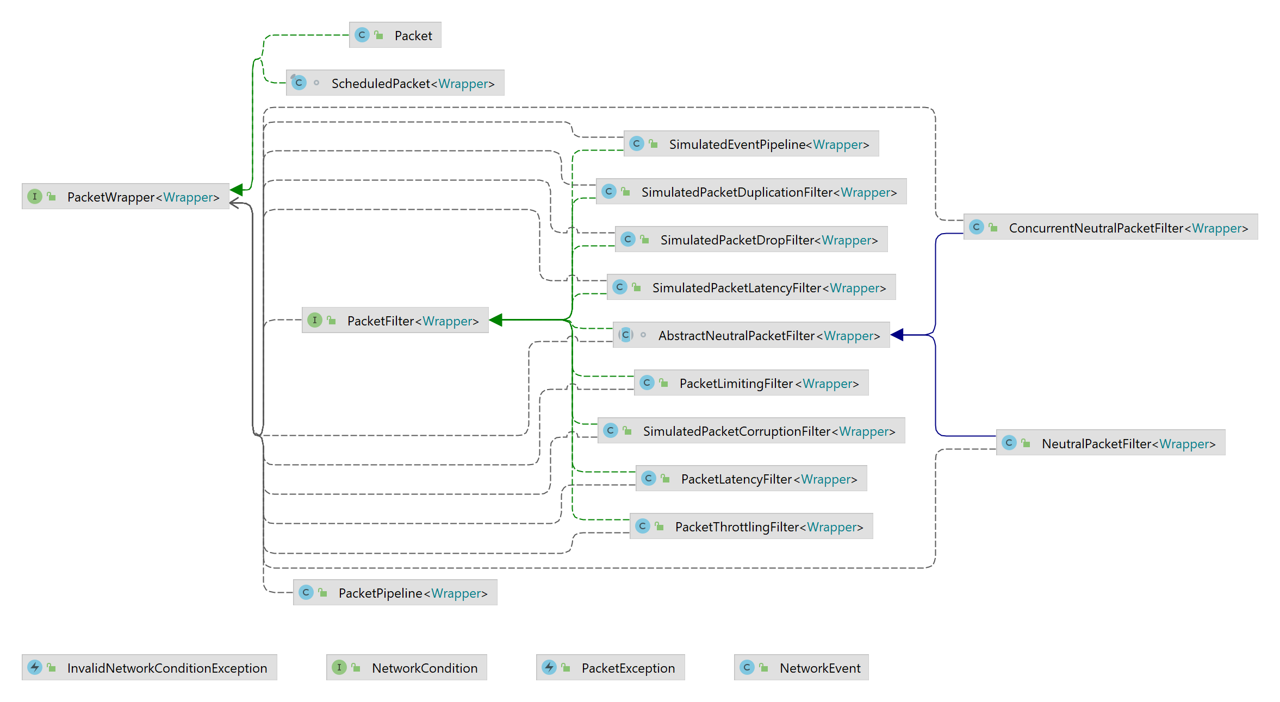
\includegraphics[width=0.8\textwidth]{images/chapter_4_implementation/network_condition_api_tree}
    \centering~\caption{A diagram showing the class inheritance tree of the network condition API.}
    \label{fig:chapter_4_implementation-network_condition_api_tree}
\end{figure}

\subsubsection{Packet \& PacketWrapper}\label{subsubsection:packet_and_packet_wrapper}

The \texttt{Packet} class is, by and large, the atomic building block for Packet Courier, despite only being a humble
wrapper for a list of bytes. A flagship feature of \texttt{Packet} is its ability to transform freely from a Java
object and back again, as demonstrated in Code-Snippet~\ref{code:packet_test}. This is achieved using Java's
\texttt{Serializable} interface\cite{java_Serializable}, which imbues inheriting classes with a canonical
representation at the level of bits; a crucial factor for communication over a wire. Furthermore, the JVM handles
serialization under-the-hood, so all a programmer needs to do is write \texttt{implements Serializable} after the
definition of a class they wish to be mailed as a \texttt{Packet}. For example, if a Packet Courier user were
simulating an authentication process using a custom class named \texttt{UserCredentials} with two \texttt{String}
attributes, \texttt{username} and \texttt{password}, then \texttt{UserCredentials} objects could be sent from worker
to worker so long as the \texttt{Serializable} interface was implemented.

\texttt{Packet} inherits from \texttt{PacketWrapper<Packet>}, a type-parameterised interface defined as follows:

\begin{lstlisting}[language=Java,caption={The \texttt{PacketWrapper<Wrapper>} interface exactly as it appears in the
codebase.},label={code:packet_wrapper_interface},captionpos=b]
public interface PacketWrapper<Wrapper extends PacketWrapper<Wrapper>> {
  Wrapper map(Function<Packet, Packet> function);

  Wrapper copy();

  Packet getPacket();
}
\end{lstlisting}


\texttt{PacketWrapper<Wrapper>} allows non-packet objects to be sent through packet pipelines. The motivation behind
this is simple: packet pipelines deal in terms of \emph{packets} and nothing else, yet there are plenty of scenarios
where users of the API might want to their packets to carry additional information as they travel through a pipeline.
The principle example within the wider context of Packet Courier is the \texttt{Mail} class, which holds the packet's
destination address for routing purposes. However, \texttt{PacketWrapper<Wrapper>} could also be used for telemetry,
instrumentation, timestamping and other broader logging purposes; any important meta-information about the packet
that users of the API might find useful.

The semantics of the \texttt{PacketWrapper<Wrapper>} interface can be likened to those of functional
homogeneity\cite{homogeneous_function}. Classes that implement \texttt{PacketWrapper<Wrapper>} provide external code
with the means to manipulate the \texttt{Packet} residing inside the wrapper without interacting with any other
aspect of the object; a similar sentiment to keyhole surgery\cite{keyhole_surgery}.

An arguably simpler solution is to use inheritance rather than composition, whereby \texttt{Mail}, say, inherits from
\texttt{Packet} and is sent through the pipeline before being cast back to \texttt{Mail} having emerged on the other
side. This is majorly inferior for many reasons:
\begin{itemize}
    \item This approach would be considered a ``hack'', since it does not make idiomatic sense within the context of
    Java. Given that \texttt{Mail} would inherit from \texttt{Packet}, then one would conclude that \texttt{Mail}
    \emph{is} a kind of \texttt{Packet}. This is not true though, in the same way that a letter isn't a type of
    envelope, but is contained within one. Indeed, as per the semantics laid out in the design document,
    \texttt{Mail} \emph{has} a \texttt{Packet}, and therefore composition is more appropriate.
    \item Casting in this way is widely agreed upon by Java programmers to be a poor practice, with excellent reasons
    to back this up\cite{reddit_casting, yegor_bugayenko_casting, mark_casting, dennis_sosnoski_casting,
        erik_dietrich_casting}.
    \item There are practical limitations to this method as well. How would more invasive packet manipulations such
    as corruption and duplication work whilst still preserving the outer class? It \emph{could} be done using
    methods such as \texttt{clone}\cite{java_clone}, but it would ultimately result in more convoluted and fragile
    code\cite{java_avoid_clone}.
\end{itemize}

\subsubsection{PacketFilter \& PacketPipeline}\label{subsubsection:packet_filter_and_packet_pipeline}

The \texttt{PacketFilter<Wrapper>} interface represents a single step in a packet pipeline and is defined as follows:
\begin{lstlisting}[language=Java,caption={The \texttt{PacketFilter<Wrapper>} interface exactly as it appears in the
codebase.},label={code:packet_filter_interface},captionpos=b]
public interface PacketFilter<Wrapper extends PacketWrapper<Wrapper>> {
  void tick(LocalDateTime now);

  void enqueue(Wrapper packetWrapper);

  Optional<Wrapper> tryDequeue();
}
\end{lstlisting}

A \texttt{PacketFilter<Wrapper>} can be conceptualised as a queue of packets that admits of special behaviour and can
be synced up with the wider simulation using the \texttt{tick} method. For example, the
\texttt{SimulatedPacketDropFilter<Wrapper>} will sample its Bernoulli distribution whenever the \texttt{enqueue}
method is called, whereby the packet is never actually enqueued if the sample is ``successful''. Another example is
the \texttt{PacketLatencyFilter<Wrapper>}\footnote{Packet filters prefixed with \texttt{Simulated} have some kind of
random component to them; conversely, filters without this prefix are deterministic and provide what could in
principle be real-world utility, such as packet throttling.} which takes instances of
\texttt{ScheduledPacket<Wrapper>} as the parameter for its \texttt{enqueue} method and stores them in a priority
queue with the packet scheduled for dequeue at the earliest time at the front of the queue. In turn,
\texttt{tryDequeue} will only release the packet at the front of the queue if a) it exists, b) its scheduled dequeue
time has passed with respect to the current simulation time; the purpose of \texttt{tick} here is to
synchronise the filter with the simulation's clock. The \texttt{NeutralPacketFilter<Wrapper>} is a simple filter with
FIFO semantics with the \texttt{ConcurrentNeutralPacketFilter<Wrapper>} being its thread-safe counterpart.

In this way, the \texttt{enqueue} and \texttt{tryDequeue} methods of packet filters can be chained together to form a
packet pipeline. In fact, this is precisely how the \texttt{PacketPipeline<Wrapper>} class works, as shown in
Code-Snippet~\ref{code:packet_pipeline_class}.
\begin{lstlisting}[language=Java,caption={A cut-down version of the \texttt{PacketPipeline<Wrapper>} class.},
    label={code:packet_pipeline_class},captionpos=b]
public class PacketPipeline<Wrapper extends PacketWrapper<Wrapper>> {
  private final List<PacketFilter<Wrapper>> packetFilters;

  private PacketPipeline(List<PacketFilter<Wrapper>> packetFilters) {
    packetFilters.add(0, new ConcurrentNeutralPacketFilter<>());
    this.packetFilters = Collections.unmodifiableList(new ArrayList<>(packetFilters));
  }

  public void enqueue(Wrapper packetWrapper) {
    packetFilters.get(0).enqueue(packetWrapper);
  }

  public void tick(LocalDateTime now) {
    for (int i = 0; i + 1 < packetFilters.size(); i++) {
      PacketFilter<Wrapper> currentFilter = packetFilters.get(i);
      PacketFilter<Wrapper> nextFilter = packetFilters.get(i + 1);
      currentFilter.tryDequeue().ifPresent(nextFilter::enqueue);
      nextFilter.tick(now);
    }
  }

  public Optional<Wrapper> tryDequeue() {
    PacketFilter<Wrapper> lastFilter = packetFilters.get(packetFilters.size() - 1);
    return lastFilter.tryDequeue();
  }
}
\end{lstlisting}

Each packet pipeline starts off with a \texttt{ConcurrentNeutralPacketFilter<Wrapper>}, not only for algorithmic ease
(i.e.: not having to do an empty check on \texttt{packetFilters} when enqueuing or dequeuing), but to ensure that
enqueuing to a packet pipeline is always a thread-safe operation. This is important because workers do their work in
parallel with one another and thus can send mail along the same channel concurrently. The \texttt{tick} and
\texttt{tryDequeue} methods needn't be thread-safe, however, which will become apparent later in this section when
their use-case is discussed.

Note that \texttt{PacketPipeline<Wrapper>} could in principle inherit from \texttt{PacketFilter<Wrapper>}, since it
implements the required methods. However, just because one could does not necessarily mean one \emph{should}. In
these circumstances, the purpose of the \texttt{PacketFilter<Wrapper>} interface is to provide developers with an API
to create and use steps in a \texttt{PacketPipeline<Wrapper>}. How would making \texttt{PacketPipeline<Wrapper>}
implement \texttt{PacketFilter<Wrapper>} be commensurate with this notion? It would enable programmers to make a
packet pipeline a step in a packet pipeline. Naturally this is a redundant and confusing API behaviour that would
only create potential for bad code.

\subsubsection{NetworkCondition}\label{subsubsection:network_condition}

The \texttt{NetworkCondition} interface acts as a \texttt{PacketFilter<Wrapper>} factory. It is important that API
users are not given the autonomy to create packet pipelines manually from packet filters or else they risk
experiencing crippling side effects. For example, a developer might decide to ``reuse'' a packet filter for two
different pipelines because the parameters are the same. This would be absolutely disastrous since packets from two
different pipelines would be routed through the \emph{same} filter, coupling them by accident and resulting in packets
going to the wrong workers. To guard against this, the only public \texttt{PacketPipeline<Wrapper>} constructor takes
an instance of the \texttt{PacketPipeline.Parameters} inner class, which is in turn a wrapper for a list of
\texttt{NetworkCondition} objects. This forces API users to create packet pipelines using abstract parameters rather
than straight from filters, delegating the creation of the actual filter instances to the pipeline itself.
\begin{lstlisting}[language=Java,caption={The \texttt{NetworkCondition} interface without any of its presets.},
    label={code:network_condition_interface},captionpos=b]
public interface NetworkCondition {
  <Wrapper extends PacketWrapper<Wrapper>> PacketFilter<Wrapper> asPacketFilterStartingAt(LocalDateTime startTime);
}
\end{lstlisting}

The \texttt{NetworkCondition} interface comes with a suite of static methods that predefine a selection of network
conditions that reflect the packet filtration mechanisms that are outlined by Packet Courier's semantics, including,
but not limited to:
\begin{itemize}
    \item \texttt{static NetworkCondition packetLimit(int packetLimitRate, ChronoUnit timeUnit)}
    \item \texttt{static NetworkCondition uniformPacketCorruption(double corruptionProbability, Random random)}
    \item \texttt{static NetworkCondition normalPacketLatency(double meanLatency, double standardDeviation,
        ChronoUnit timeUnit, Random random)}
\end{itemize}

\subsubsection{SimulatedEventPipeline}\label{subsubsection:simulated_event_pipeline}

The \texttt{SimulatedEventPipeline<Wrapper>} class is a packet filter that implements the event-based semantics
outlined in the design documentation. It is the only \texttt{PacketFilter<Wrapper>} that will be specifically
discussed because it is notably more complicated than the others. The attributes of
\texttt{SimulatedEventPipeline<Wrapper>} are listed in
Code-Snippet~\ref{code:simulated_event_pipeline_class_attributes}.
\begin{lstlisting}[language=Java,caption={The attributes of the \texttt{SimulatedEventPipeline<Wrapper>} class.},
    label={code:simulated_event_pipeline_class_attributes},captionpos=b]
public class SimulatedEventPipeline<Wrapper extends PacketWrapper<Wrapper>> implements PacketFilter<Wrapper> {
  private final List<State> states;
  private final StateTracker stateTracker;
  private final PriorityQueue<ScheduledEvent> eventQueue = new PriorityQueue<>();
  private final NeutralPacketFilter<Wrapper> outputBuffer;
  private final ChronoUnit timeUnit;
  private final Random random;
  private LocalDateTime now;

  // Rest of class...
}
\end{lstlisting}

In essence, a \texttt{SimulatedEventPipeline<Wrapper>} juggles multiple packet pipelines which correspond to network
events and is responsible for scheduling which \texttt{PacketPipeline<Wrapper>} is currently ``active'', i.e.:
having packets enqueued to it. As such, each \texttt{State} contains a live packet pipeline, a unique precedence
value and the mean interval and duration of their associated network event. The \texttt{StateTracker} keeps
track of which network events are currently happening and which has the highest precedence; this helps the
\texttt{enqueue} method decide which pipeline the given packet should go to. Java's Red-Black tree implementation,
\texttt{TreeSet}\cite{java_TreeSet, baeldung_java_TreeSet}, is used to achieve this behaviour; it is used instead of
\texttt{PriorityQueue} because it guarantees logarithmic removal times for an arbitrary element, whereas
\texttt{PriorityQueue} requires linear time for this operation\cite{java_PriorityQueue}.

The \texttt{eventQueue} tracks the timeline of events, i.e.: when each network event starts and finishes. When a
\texttt{ScheduledEvent} starts, its respective state is pushed to the \texttt{stateTracker}; conversely, when a
\texttt{ScheduledEvent} finishes, its respective state is popped from the \texttt{stateTracker}. Note that the
\texttt{stateTracker} will never ``run out'' of states since the class is always given a set of default network
conditions, which in turn form the basis for a ``default state''.

The \texttt{states} attribute contains all possible states that could be active, i.e.: the default state plus a state
for each network event. This is used in the \texttt{tick} method to ensure that each packet pipeline is synchronised.
Similarly, the \texttt{tryDequeue} method also calls \texttt{tryDequeue} on each packet pipeline in \texttt{states}
and siphons off any dequeued packets to the \texttt{outputBuffer}, which is then itself dequeued for the value
that is ultimately returned. Indeed, \texttt{outputBuffer} is simply a way to linearize the outputs of the multiple
packet pipelines being used.

It is important to note that \texttt{tryDequeue} isn't implemented by simply calling \texttt{tryDequeue} on the current
state. This is because packets may still exist within a packet pipeline ``in transit'' even after the network event is
over and those packets should still be delivered. Consider a network event that occurs every 300 seconds and lasts
for 10 seconds (on average) and adds a flat 75-second latency to each packet. If the packets in this particular
pipeline are only dequeued when their state is active, then the packets will have a latency of 300 seconds as opposed
to 75, since the 10-second duration of the event is not long enough to see them dequeued from their packet pipeline
and the next time the state will become active again is in 300 seconds, meanwhile the packets are stuck in memory!

\subsection{Worker API}\label{subsection:worker_api}

\begin{figure}[!h]
    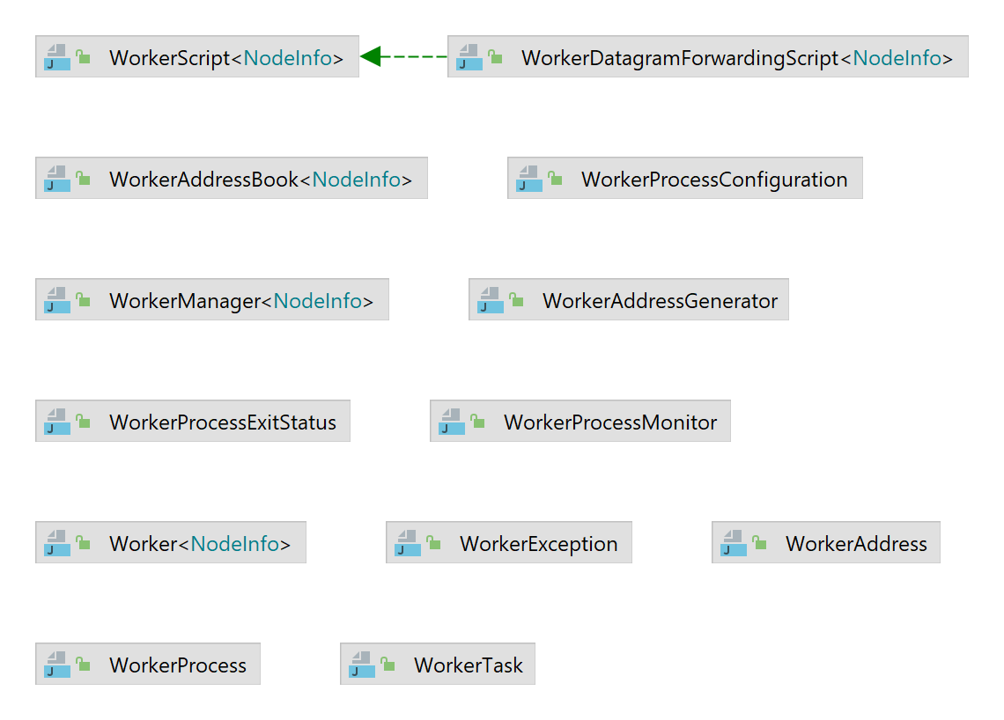
\includegraphics[width=0.65\textwidth]{images/chapter_4_implementation/worker_api_tree}
    \centering~\caption{A diagram showing the class inheritance tree of the worker API. Some of these classes are
    specific to Packet Courier's emulator functionality and thus will be discussed in
    Section~\ref{section:standalone_emulator}.}
    \label{fig:chapter_4_implementation-worker_api_tree}
\end{figure}

\subsubsection{Worker}\label{subsubsection:worker}

As described in the Section~\ref{subsection:simulation_semantics}, a Packet Courier worker is simply an agent within
the simulation that performs work and is owned by a particular node. The \texttt{Worker<NodeInfo>} class is
implemented as a wrapper for a Java \texttt{Thread}\cite{java_Thread} with a couple of useful abstractions layered on
top.
\begin{lstlisting}[language=Java,caption={A cut-down version of the \texttt{Worker<NodeInfo>} class.},
    label={code:worker_class},captionpos=b]
public class Worker<NodeInfo> {

  private final Thread workerThread;
  private final WorkerAddress address;
  private final Mailbox mailbox;
  private State state;

  // Rest of class...

  public enum State {
    READY,
    RUNNING,
    DEAD
  }
}
\end{lstlisting}

Just as with a Java \texttt{Thread}\cite{java_Thread}, \texttt{Worker<NodeInfo>} has methods \texttt{run},
\texttt{start}, \texttt{join} and \texttt{interrupt} which enjoy similar semantics, although the states are massively
simplified. Note that unlike with \texttt{Thread}, the \texttt{join} method in \texttt{Worker<NodeInfo>} does not
have \texttt{throws InterruptedException} in its type signature, instead opting to a throw a \texttt{WorkerException}
which inherits form \texttt{RuntimeException}\cite{java_RuntimeException}. This was a deliberate design decision to
discourage API users to rely on the \texttt{interrupt} mechanic as it creates complex inter-worker behaviours. The
idea behind the \texttt{Worker<NodeInfo>} class is \emph{not} to be a thread in disguise, but rather to enable work
to be done in parallel on each node. In principle, a worker should start, do its work, then finish with minimal fuss.
Indeed, cutting out the potential for an \texttt{InterruptedException} in turn removes the mandate for a try-catch
around every invocation of \texttt{join}, making for cleaner worker scripts.

\texttt{Worker<NodeInfo>} also has a public \texttt{post} method which allows external code to insert a
\texttt{Packet} into the worker's \texttt{Mailbox}. In the wider context of Packet Courier, a strict privacy
hierarchy forms with respect to who can post into which mailbox, i.e.: a node can deliver\footnote{Insofar as
``deliver'' means to post directly; any worker can \emph{mail} a packet to any other worker so long as they have the
correct address and their respective nodes are topologically connected.} mail to any worker in its command and a
worker can deliver mail to its children.

\subsubsection{WorkerAddress, WorkerAddressGenerator \&
WorkerAddressBook}\label{subsubsection:worker_address_worker_address_generator_and_worker_address_book}

The \texttt{WorkerAddress} class simply provides each \texttt{Worker} with a way of being uniquely identified. It
also implements \texttt{Serializable}\cite{java_Serializable} so that it can be over the wire, allowing workers to
distribute their address. Each worker is given a \texttt{name} in the form of a \texttt{String}
attribute, but this is only unique with respect to the hosting node. For example, two nodes Alice and Bob
could have workers with the same \texttt{name}. As a consequence each \texttt{WorkerAddress} also tracks the address
of its hosting node to supplement this, making each instance of \texttt{WorkerAddress} truly unique. It is doubly
crucial that a \texttt{WorkerAddress} contains the \texttt{NodeAddress} of the hosting node so that the postal
service knows where to route \texttt{Mail} to.

Note that every instance of \texttt{WorkerAddress} has access to its parent address as well. Whilst this isn't
necessary to make the address unique, it is a useful addition. Indeed, it makes sense that nodes might want to hide
information from one another, or perhaps even different workers on the same node, yet there is little justification
for a parent worker hiding its address from its child. To follow through with the real-world analogy laid out in the
design where a node represents a router and a worker represents a machine, then this would be the equivalent of a
machine hiding its ip-address from its own virtual machine. This could in theory be for security reasons, although
that isn't necessarily applicable in the context of a Packet Courier simulation. If a worker spawns a child worker,
then it is by definition because it wants it to do some work for it. In that case, it is likely that the parent will
want to receive some communication from the child, at which point why not just cut out the extra step of the parent
and child having to do an initial handshake where the parent gives the child its address?

\texttt{WorkerAddressGenerator} leverages a utility class that was developed in-house, \texttt{UniqueStringGenerator},
to generate unique worker names. It does so using the simple algorithm of adding a prefix to a counter that
increments with each new generation and lengthening the prefix when the counter overflows.

\texttt{WorkerAddressBook<NodeInfo>} is used by nodes to keep track of their workers, taking advantage of Java's
\texttt{ConcurrentHashMap}\cite{java_ConcurrentHashMap} to link workers with their addresses. Naturally, this allows
nodes to route mail to their workers based on the destination address. There are two critical abstractions that
\texttt{WorkerAddressBook} distinct from a simple map.

First and foremost there is a garbage collection component to tracking workers, since they have a tendency to die
off. If dead workers were never removed from a \texttt{WorkerAddressBook<NodeInfo>}, then this would quickly become a
black hole with respect to memory. Packet Courier tackles this issue by using a custom design pattern that combines
an in-house \texttt{Prunable} interface with a \texttt{GarbageCollector} which automatically remove dead workers from a
\texttt{WorkerAddressBook} on every tenth address lookup.

The second key abstraction comes in the form of the \texttt{registerWorker} method which creates a worker and adds it
to the \texttt{addressToWorkerMap} before returning it. In fact, \texttt{WorkerAddressBook<NodeInfo>} is the only
class in the entire Packet Courier codebase that creates instances of \texttt{Worker<NodeInfo>} from scratch,
ensuring that any new workers are logged in a relevant address book.

\subsubsection{WorkerManager \& WorkerScript}\label{subsubsection:worker_manager_and_worker_script}

The \texttt{WorkerManager<NodeInfo>} class is where most of the magic happens regarding the worker API. As per the
semantics presented in Section~\ref{subsection:application_programmer_interface}, it is the black box that enables a
worker to interact with the wider simulation. In this way, a \texttt{WorkerScript<NodeInfo>} is defined as in
Code-Snippet~\ref{code:worker_script_interface}.
\begin{lstlisting}[language=Java,caption={The \texttt{WorkerScript<NodeInfo>} interface exactly as it appears in the
codebase.},label={code:worker_script_interface},captionpos=b]
@FunctionalInterface
public interface WorkerScript<NodeInfo> {
  void run(WorkerManager<NodeInfo> workerManager);
}
\end{lstlisting}

Despite the pivotal role it plays in providing users with the abstraction of writing code for an arbitrary worker,
the \texttt{WorkerManager<NodeInfo>} class itself is relatively uncomplicated and simply houses a collection of key
components that a worker may need to use indirectly, such as its \texttt{Mailbox}, \texttt{NodeInfo} and the
simulation \texttt{PostalService}. This abstraction is important from a software engineering perspective as well,
since it protects these components from being used in ways that might break the semantics of the simulation through
encapsulation leakage. For example, the \texttt{PostalService} interface enables developers to send mail from a
source to a destination, but if this was provided to a worker outright, then the worker could in turn spoof the
source address: it is this kind of behaviour that the \texttt{WorkerManager<NodeInfo>} protects against.

\subsubsection{WorkerTask}\label{subsubsection:worker_task}

A \texttt{WorkerTask} is a simple abstraction that allows Packet Courier API users to write code times out in an
elegant fashion. See Code-Snipet~\ref{code:worker_task_example} for an example.
\begin{lstlisting}[language=Java,caption={An example of how \texttt{WorkerTask} might be used.},
    label={code:worker_task_example},captionpos=b]
public class WorkerTaskExample {
  public static void myWorkerScript(WorkerManager<WorkerTaskExampleNodeInfo> workerManager) {
    WorkerTask.configure()
        .withTimeout(5, TimeUnit.SECONDS)
        .execute(
            () -> {
              // Do some work.
            });
  }
}
\end{lstlisting}

\subsection{Node API}\label{subsection:node_api}

\lettrine{W}{hen} compared to the worker API, the node API is somewhat straightforward. In fact, the
\texttt{network.simulation.node} package only contains an interface and four classes which in turn are mostly
data-oriented. For example, Code-Snippet~\ref{code:node_class} details the majority of functionality implemented by
the \texttt{Node<NodeInfo>} class. It is however missing the methods \texttt{doWork}, \texttt{hashCode} and
\texttt{equals}, but these are fairly trivial implementations. As one might expect, \texttt{doWork} is used to
initiate the root worker. Whilst in principle the API has the capacity to have multiple root workers do work, it is
limited to one for simplicity. \begin{lstlisting}[language=Java,caption={A cut-down version of the
\texttt{Node<NodeInfo>} class.},label={code:node_class},captionpos=b]
public class Node<NodeInfo> {
  private final NodeAddress address;
  private final WorkerAddressGenerator workerAddressGenerator;
  private final WorkerAddressBook<NodeInfo> workerAddressBook;

  public void deliver(Mail mail) {
    workerAddressBook
        .lookup(mail.getDestinationAddress())
        .ifPresent(worker -> worker.post(mail.getPacket()));
  }
}
\end{lstlisting}

The \texttt{NodeAddress} class wraps a \texttt{String} attribute \texttt{name} which is provided and guaranteed to be
unique by the user. It also provides some additional utility, such as \texttt{asRootWorkerAddress} and a custom
\texttt{toString} method. \texttt{NodeConnection<NodeInfo>} is similar in that it bundles two \texttt{Node<NodeInfo>}
attributes together: \texttt{source} and \texttt{destination}.

The most interesting aspect of the node API is the \texttt{NodeInfoGenerator<NodeInfo>} interface which is defined in
Code-Snippet~\ref{code:node_info_generator_interface}. It is this component that allows users to define what
information workers in their simulation have access to. As per
Section~\ref{subsection:application_programmer_interface}, each node generates its own info-package on simulation
startup which then gets handed out to each worker operating on that particular node. This is why many of the classes
and interfaces in the node and worker APIs are type parameterised by \texttt{NodeInfo}.
\begin{lstlisting}[language=Java,caption={The \texttt{NodeInfoGenerator<NodeInfo>} interface exactly as it appears in
the
codebase.},label={code:node_info_generator_interface},captionpos=b]
@FunctionalInterface
public interface NodeInfoGenerator<NodeInfo> {
  NodeInfo generateInfo(NodeAddress address, Topology topology, Clock clock);
}
\end{lstlisting}

\texttt{DefaultNodeInfo} is provided as a sensible default for users who might not need anything especially bespoke
for their simulation. It provides each worker with access to the addresses of the neighbouring nodes and the current
simulation time.

\subsection{Mail API}\label{subsection:mail_api}

\lettrine{A}{s} with the node API, the mail API is fairly data focused. For example, the \texttt{Mail} class is
composed of a \texttt{Packet} and a destination \texttt{WorkerAddress}. It is Packet Courier's chosen mode of
transport of packets and thus inherits from \texttt{PacketWrapper<Mail>} so that it can travel along instances of
\texttt{PacketPipeline<Mail>}.

The \texttt{Mailbox} class is a wrapper for Java's \texttt{LinkedBlockingQueue}\cite{java_LinkedBlockingQueue}: a
thread-safe queue that makes the polling thread wait until a new element is available. The renaming of elements alone
is useful for abstraction purposes, as well it being an instance of an Adapter pattern\cite{adapter_pattern}.

\texttt{PacketCourierPostalService<NodeInfo>} implements the \texttt{PostalService} interface which is defined in
Code-Snippet~\ref{code:postal_service_interface} and is responsible for routing and delivering packets. It uses two
maps to achieve this:
\begin{itemize}
    \item \texttt{Map<NodeAddress, Node<NodeInfo>> nodeToAddressMap}
    \item \texttt{ConcurrentMap<NodeConnection<NodeInfo>, PacketPipeline<Mail>>}
    \texttt{nodeConnectionToPacketPipelineMap}
\end{itemize}

Naturally, the \texttt{mail} method is implemented by looking up the respective nodes of the source and destination
worker addresses using the \texttt{nodeToAddressMap} and in turn using them to formulate a
\texttt{NodeConnection<NodeInfo>} which can then used to get the respective \texttt{PacketPipeline<Mail>} from
\texttt{nodeConnectionToPacketPipelineMap}. The given packet is then packaged up as \texttt{Mail} with the
destination address and enqueued into the relevant packet pipeline.

The \texttt{PacketCourierPostalService<NodeInfo>} class also has a \texttt{tick} method which calls \texttt{tick} on
each of the pipelines in \texttt{nodeConnectionToPacketPipelineMap} before forwarding any dequeued packets to their
destination node.

\begin{lstlisting}[language=Java,caption={The \texttt{PostalService} interface exactly as it appears in the
codebase.},label={code:postal_service_interface},captionpos=b]
public interface PostalService {
  boolean mail(WorkerAddress sourceAddress, WorkerAddress destinationAddress, Packet packet);
}
\end{lstlisting}

\subsection{Simulation API}\label{subsection:simulation_api}

\lettrine{T}{he} \texttt{PacketCourierSimulation<NodeInfo>} class brings all the elements discussed thus far together
to build a fully functioning simulation. An API user would configure their simulation using the
\texttt{Configuration<NodeInfo>} inner class which leverages a builder pattern\cite{builder_pattern}. This allows the
user to add nodes, connections, network conditions and other peripheral elements such as logging mechanisms to their
simulation in a way that is easy and human readable. Once they have built their simulation, they can then run it
using the \texttt{start} method which runs asynchronously and can be joint back to the current thread using
\texttt{waitFor}, mirroring the semantics of Java's \texttt{Process} class\cite{java_Process}.

The main responsibility of the \texttt{PacketCourierSimulation<NodeInfo>} is to correctly manage the various
components that make up a simulation, rather than provide any novel functionality. A bare-bones Packet Courier
simulation will involve the following steps:
\begin{enumerate}
    \item Collect configuration information from the user.
    \item Build a postal service.
    \item Upon startup, create a thread for each node which sets them to work.
    \item Create a management thread to tick the simulation clock and the postal service.
    \item Start all threads.
    \item Wait on the node threads to finish.
    \item Mark the simulation as complete and wait for the management thread to finish.
    \item Flush and close the loggers.
\end{enumerate}

\begin{lstlisting}[language=Java,caption={An example of how a \texttt{PacketCourierSimulation<NodeInfo>} might be set
up and used.},
    label={code:simulation_example},captionpos=b]
public class PacketCourierSimulationExample {

  public static final String NODE_A_NAME = "Alice";
  public static final String NODE_B_NAME = "Bob";

  public static void aliceWorkerScript(WorkerManager<DefaultNodeInfo> workerManager) {
    // Alice does some work.
  }

  public static void bobWorkerScript(WorkerManager<DefaultNodeInfo> workerManager) {
    // Bob does some work.
  }

  public static void main(String[] args) {
    Random random = new Random(42);
    PacketCourierSimulation<DefaultNodeInfo> packetCourierSimulation =
        PacketCourierSimulation.configuration()
            .addNode(NODE_A_NAME, PacketCourierSimulationExample::aliceWorkerScript)
            .addNode(NODE_B_NAME, PacketCourierSimulationExample::bobWorkerScript)
            .addConnection(
                NODE_A_NAME,
                NODE_B_NAME,
                PacketPipeline.parameters(
                    NetworkCondition.uniformPacketDrop(0.5, random),
                    NetworkCondition.uniformPacketLatency(
                        35.0, 50.0, ChronoUnit.MILLIS, random)))
            .addLogger(ConsoleLogger.out())
            .configure();
    packetCourierSimulation.start();
    try {
      packetCourierSimulation.waitFor();
    } catch (InterruptedException e) {
      e.printStackTrace();
    }
  }
}
\end{lstlisting}

\newpage

\begin{lstlisting}[language=Java,caption={A \emph{massively} cut-down version of the
\texttt{PacketCourierSimulation<NodeInfo>} class.},
    label={code:simulation_class},captionpos=b]
public class PacketCourierSimulation<NodeInfo> {
  // There is a fair amount of instrumentation that has been left out for simplicity's sake.
  private void run(
      Map<String, RunnableNode<NodeInfo>> nodes,
      PacketCourierPostalService<NodeInfo> postalService,
      Clock clock,
      Logger logger) {
    AtomicBoolean simulationComplete = new AtomicBoolean(false);
    // This is not a real method, of course - the actual code is just too long!
    Map<Node<NodeInfo>, Thread> nodeThreads = getNodeThreadsSomehowFrom(nodes);
    Thread simulationManagerThread =
        new Thread(
            () -> {
              while (!simulationComplete.get()) {
                clock.tick();
                postalService.tick(clock.now());
              }
            });
    nodeThreads.values().forEach(Thread::start);
    simulationManagerThread.start();
    joinAll(nodeThreads.values());
    simulationComplete.set(true);
    try {
      simulationManagerThread.join();
    } catch (InterruptedException e) {
      // Handle exception.
    }
    logger.flush();
    logger.close();
  }
}
\end{lstlisting}

The last piece of the puzzle is the \texttt{Clock} interface, as defined in Code-Snippet~\ref{code:clock_interface}.

\begin{lstlisting}[language=Java,caption={The \texttt{Clock} interface exactly as it appears in the codebase.},
    label={code:clock_interface},captionpos=b]
public interface Clock {
  void tick();

  LocalDateTime now();
}
\end{lstlisting}

There are two classes that inherit from \texttt{Clock}: \texttt{VirtualClock} and \texttt{WallClock}; herein lies the
key distinction between a simulation and an emulation. When the \texttt{VirtualClock} ticks over, it simply adds an
arbitrary unit of time to a counter. Given that each worker runs on its own thread, one could think of a
\texttt{VirtualClock} tick as a simulation time slice or \emph{quantum}\cite{cpu_time_slicing} on the assumption that
CPU scheduling is fair. In theory this provides Packet Courier simulations with perfect scaling, because although
adding an extra worker will mean that more computational resources are required, the CPU scheduler will ensure that
all threads will enjoy roughly the same amount of CPU time. In turn, this provides the illusion of total parallelism,
since each worker will work for a simulation quantum before the simulation clock ticks over.

Packet Courier's \texttt{VirtualClock} keeps track of a \texttt{LocalDateTime}\cite{java_LocalDateTime} that is
initialized to midnight on the 1\textsuperscript{st} of January, Year 0. This value has a single unit of time added
to it on each call to \texttt{tick}, namely a \texttt{ChronoUnit}\cite{java_ChronoUnit} of the user's choosing. For
example, if the user specifies a flat latency of 42 milliseconds between Alice and Bob, then this could be 42
or 42,000 \texttt{VirtualClock} ticks depending on the given unit. API users might indeed find that they need to do
some hyperparameter tuning to find the unit of granularity that suits their simulation, since \texttt{VirtualClock}
ticks can be extremely short with respect to real-time (as low as a few hundred nanoseconds). For instance, if worker
Charlie is connected to Alice with a normally distributed latency with a mean of 42 milliseconds (arbitrary
unit set by the user) and sends her a packet approximately every real millisecond of CPU time, but a simulation
quantum is about one real microsecond of CPU time, then Charlie is sending a packet to Alice every 1000 ticks.
Indeed, if one tick is programmed to represent one millisecond for abstraction purposes, then the probability of
packets being reordered when being sent from Charlie to Alice is virtually zero, but the user may expect a certain
degree of reordering due to the random latency they have specified. It is ``gotchas'' like these that are important
to consider when using Packet Courier for simulation.

\emph{Emulation}, on the other hand, is an entirely different beast and uses a \texttt{WallClock} instead. As one
might imagine, the \texttt{tick} method in \texttt{WallClock} does nothing since the \texttt{now} method just
retrieves the current wall time. This seemingly small change results in wholesale different behaviour, i.e.: Alice's
42-millisecond delay when sending packets to Bob will actually be 42 milliseconds, as opposed to 42 milliseconds in a
virtual or simulated sense.


\section{Standalone Emulator}\label{section:standalone_emulator}

\lettrine{P}{acket} Courier achieves language agnosticism by offering UDP interoperability. As a consequence, any
binary that uses UDP (directly or indirectly) to send and receive packets can enjoy what the Packet Courier API has
to offer. This is achieved by giving each node a pair of public and private ip-addresses and opening a UDP socket for
each public ip-address, as per the emulation semantics outlined in Section~\ref{subsection:emulation_semantics}.

Packet Courier users can in principle mix and match the API with the UDP adaptive solution, i.e.: have workers that
use custom Java code and nodes that are communicating with a binary over UDP \emph{in the same simulation/emulation}.
The limitation with this approach is that UDP sockets are assigned on a node-by-node basis, not worker-by-worker. As
such, if a Packet Courier node Alice has workers Charlie and Doris, but node Bob is using an arbitrary binary, then
Bob's binary could send UDP packets to Alice, but not Charlie or Doris. In theory workers could be given UDP
sockets on-the-fly, although this would be a potential feature for the future.

Mixing and matching API and UDP functionality like this would be unusual, though; the most common use-cases would be
simulation via the API and emulation via UDP. In the case where Packet Courier's UDP functionality is used for
emulation, it will run silently in the background while other processes communicate through it, treating it as though
it were an authentic physical network. At that point, the next logical step is to provide users with the option to
never write any Java code at all, i.e.: they configure the network they want via some portable, high-level
configuration file and spin-up a Packet Courier emulation from the command-line. This is exactly what the standalone
Packet Courier emulator does.

\subsection{Key Components}\label{subsection:key_components}

\subsubsection{WorkerProcess, WorkerProcessConfiguration \&
WorkerProcessExitStatus}\label{subsubsection:worker_process_worker_process_configuration_and_worker_process_exit_status}

A \texttt{WorkerProcess} is a wrapper for a Java \texttt{Process}\cite{java_Process} that enables Packet Courier to
invoke commands within the user space of the host operating system. The exact nature of the command is subject to
change based on the node, however, which is why a suite of environment variables are available so that users can
inject runtime data into their commands:
\begin{itemize}
    \item \texttt{NODE\_NAME} \\
    Corresponds to the name that either the configuration file or Packet Courier has assigned to the node running the
    command.
    \item \texttt{PUBLIC\_IP} \\
    Corresponds to this node's public ip-address, i.e.: the address that other nodes should send packets to if they
    want Packet Courier to route it back to this node. Similar to a PO Box address.
    \item \texttt{PRIVATE\_IP} \\
    Corresponds to the node's private ip-address, i.e.: the address that this node should listen on to receive
    packets. Similar to a house address.
    \item \texttt{PORT} \\
    Corresponds to the port that nodes have been configured to listen on.
    \item \texttt{DATAGRAM\_BUFFER\_SIZE} \\
    Corresponds to the buffer size of the UDP sockets that Packet Courier is listening on.
    \item \texttt{NEIGHBOUR\_IPS} \\
    Corresponds to the names and public ip-addresses of neighbouring nodes.
    \item \texttt{FLOOD\_IPS\_BY\_DISTANCE=[distance]} \\
    Generates the names and public ip-addresses of a basic flood search with search radius \texttt{distance}.
    \item \texttt{TOPOLOGY\_IPS} \\
    Corresponds to the names and public ip-addresses of the entire topology, including nodes that this node isn't
    adjacent to and therefore cannot communicate with directly.
\end{itemize}

For example, if Alice and Bob were configured to be bidirectionally connected, listening on port 1234 with a datagram
buffer size of 128, then Alice's command:
\begin{quote}
    \texttt{python3 server.py \$\{NODE\_NAME\} \$\{PORT\} \$\{DATAGRAM\_BUFFER\_SIZE\}}
    \texttt{\$\{PRIVATE\_IP\} \$\{PUBLIC\_IP\}} \texttt{\$\{NEIGHBOUR\_IPS\}}
\end{quote}
\noindent
\ldots would be translated at runtime into something like:
\begin{quote}
    \texttt{python3 server.py Alice 1234 128 127.0.0.3 127.0.0.4 \{"Bob": "127.0.0.6"\}}
\end{quote}

Note that this feature uses environment variable notation as an easy convention, but these are not actually
environment variables at the level of the operating system. A real environment variable such as
\texttt{\$\{JAVA\_HOME\}} would not be translated into something like \texttt{/usr/lib/jvm/java-8-oracle} at runtime.

The \texttt{WorkerProcessConfiguration} handles the string processing required to find and replace the relevant
environment variables, doing so by splitting the command based on whitespace and then examining each resulting word
using Java's in-built regex matching libraries \texttt{Pattern}\cite{java_Pattern} and
\texttt{Matcher}\cite{java_Matcher}.

A \texttt{WorkerProcessConfiguration} is then converted into a \texttt{WorkerProcess.Factory} via the
\texttt{buildFactory} method, which takes in runtime variables such as \texttt{Map<WorkerAddress, InetAddress>
    workerAddressToPublicIpMap} to determine the values associated with the environment variables. In turn,
\texttt{WorkerProcess.Factory} is essentially a wrapper for Java's \texttt{ProcessBuilder}\cite{java_ProcessBuilder}.
The \texttt{WorkerProcess.Factory} has a \texttt{start} method which triggers the associated \texttt{Process} and
returns an encapsulating \texttt{WorkerProcess}.

\texttt{WorkerProcess} has a method called \texttt{waitFor} which spawns a thread that actively listens for console
output from the running process. Even if process logging has been disabled by the user, it is still important to
empty the process's output buffer since Java processes have been known to hang when their I/O buffers fill
up\cite{java_process_hang_due_to_buffer_overflow}. The \texttt{waitFor} method does some final tidying up of
resources once its Java process has finished before returning a \texttt{WorkerProcessExitStatus}, which indicates to
the calling code whether the process finished successfully or with a failure, detailing any relevant error messages.

\subsubsection{WorkerDatagramForwardingScript}\label{subsubsection:worker_datagram_forwarding_script}

The \texttt{WorkerDatagramForwardingScript<NodeInfo>} class implements the\texttt{WorkerScript <NodeInfo>} interface
and thus can be run by a worker straight out of the box, whereby its key responsibilities are:
\begin{itemize}
    \item To run and manage the \texttt{WorkerProcess} for the current node.
    \item To forward any Packet Courier \texttt{Mail} to the private ip-address of the process.
\end{itemize}

The second task is surprisingly non trivial. The crucial difficulty is that the recipient needs to be provided with
the illusion that the packet was sent from the sender's public ip-address, but a key aspect of the Packet Courier's
semantics are that the workers don't know the \texttt{WorkerAddress} of the sender by default. This issue is solved
by smuggling the private ip-address of the sender through the packet pipeline by appending into onto the last four
bytes of the packet\footnote{This means it could be corrupted during transit}. Once the packet arrives, the sender's
public UDP socket is looked up based on its private ip-address via the \texttt{privateIpAddressToPublicSocketMap}
attribute in \texttt{WorkerDatagramForwardingScript<NodeInfo>}. The packet contents (i.e.: without the appended
ip-address) are then sent to current node's private ip-address via the sender's public UDP socket.

\subsubsection{PacketCourierSimulation}\label{subsubsection:packet_courier_simulation}

The main simulation class contributes a substantial amount of work towards the standalone emulator, whereby its key
responsibilities are:
\begin{itemize}
    \item To generate batch of unique private and public ip-addresses, i.e.: one of each for every node.
    \item To create a \texttt{DatagramSocket}\cite{java_DatagramSocket} for each public ip-address.
    \item To build and maintain a \texttt{privateIpAddressToWorkerAddressMap}, which is used in the
    \texttt{listenForAndRouteDatagramPackets} method.
    \item To build and maintain a \texttt{publicIpAddressToWorkerAddressMap}, which is also used in the
    \texttt{listenForAndRouteDatagramPackets} method.
    \item To build and maintain a \texttt{privateIpAddressToPublicSocketMap}, which is used in
    \texttt{WorkerDatagramForwardingScript<NodeInfo>}.
    \item To build and maintain a \texttt{workerAddressToPublicIpMap}, which is used by
    \texttt{WorkerProcessConfiguration} to build a \texttt{WorkerProcess.Factory}.
    \item To build and maintain a \texttt{nodeToPublicSocketMap}, which is used in the main simulation body.
\end{itemize}

Each public UDP socket has a thread that runs the \texttt{listenForAndRouteDatagramPackets} method, which in turn
listens on the given public UDP socket and converts the received packet into a format that can be sent by the postal
service; namely by getting the worker addresses of the private source-ip and public destination-ip using the relevant
maps.

\subsection{Protocol Buffer Integration}\label{subsection:protocol_buffer_integration}

\lettrine{P}{acket} Courier uses Google's Protocol Buffer library\cite{google_protobuf} to define configuration syntax
for files that in turn outline the parameters for an emulation, as per
Section~\ref{subsubsection:google_protocol_buffer}. The full syntax and semantics of Packet Courier's \texttt{
    .courierconfig} file can be found in the \texttt{README.md} of the GitHub repository\cite{packet_courier}. At a
technical level, the Protocol Buffer library is used to convert the file into a parse-tree which is then traversed by
the \texttt{PacketCourierSimulationConfigurationProtoParser<NodeInfo>} class to then build a
\texttt{PacketCourierSimulation.Configuration<NodeInfo>} from scratch. This combined with the
\texttt{PacketCourierMain} class enables users to run an emulation from the command line without having to write a
single line of Java code via the following process:
\begin{quote}
    \texttt{> cd path/to/packet/courier/root/} \\
    \texttt{> mvn package -DskipTests} \\
    \texttt{> java -jar "target/packet-courier-[version].jar"} \\ \texttt{"path/to/configuration\_file.courierconfig"}
\end{quote}


\section{Debugging Features}\label{section:debugging_features}

\lettrine{P}{acket} Courier implements a suite of debugging features to help developers understand what is happening
within Packet Courier itself without needing to consult a lower level code debugging tool such as
\texttt{jdb}\cite{jdb}.

\subsection{Meta Logging}\label{subsection:meta_logging}

\lettrine{T}{he} \texttt{Logger} interface has not been discussed thus far in the report and that has been because the
API that surrounds it is elementary. Packet Courier loggers simply provide users with a clean and easy mechanism to
track output from workers. \emph{Meta logging}, however, does not involve workers at all and instead enables the
Packet Courier internals to log meaningful information. For example, Packet Courier is instrumented to measure the
average time it takes to execute a simulation tick; the result is periodically \emph{meta logged}. Other more
procedural information is meta logged as well, such as which nodes have been set to work and when, when the
simulation has finished and when the loggers are being flushed and closed. If Packet Courier happened to crash for
whatever reason, then meta logging may help to identify when the crash occurred and what might have caused it.

\newpage

\subsection{Process Monitor}\label{subsection:process_monitor}

\lettrine{T}{he} \texttt{WorkerProcessMonitor} class goes a step further than the meta logging feature and starts a
thread which periodically checks the status of each running child \texttt{Process}\cite{java_Process}. Users can
specify how often the process monitor should perform its checks, which involve meta logging which processes are still
alive and which have finished since its last check. This can be very useful for users who might want to find out why
their simulation is hanging, i.e.: which processes aren't finishing of their accord.

\subsection{Crash Dumps}\label{subsection:crash_dumps}

\lettrine{U}{sers} can specify a crash dump path for instances when processes end unceremoniously. By default, such
errors will be logged via the traditional chancels, but adding a crash dump path will siphon them away to a separate,
discreet file and thereby keeping the man logs clean.
